% =====================================================================
% CS769 project report
% Multi-objective Optimisation for Multilingual Tokenization
% Compile with pdfLaTeX. Self-contained: no .bib file and no data files.
% =====================================================================
\documentclass[11pt,a4paper]{article}
\usepackage[T1]{fontenc}
\usepackage[utf8]{inputenc}
\usepackage{mathptmx}  % Times text and maths; available everywhere
\usepackage[scaled=0.9]{helvet}
\usepackage[margin=2.4cm]{geometry}
\usepackage{amsmath,amssymb,amsthm}
\usepackage{booktabs}
\usepackage{graphicx}
\usepackage{xcolor}
\usepackage{pgfplots}
\pgfplotsset{compat=1.18}
\usepackage[font=small,labelfont=bf]{caption}
\usepackage{microtype}
\usepackage[hidelinks]{hyperref}

\definecolor{pfair}{HTML}{0B3D91}
\definecolor{hybrid}{HTML}{D9622B}
\definecolor{soft}{HTML}{DDE3EC}

\newtheorem{proposition}{Proposition}
\theoremstyle{remark}
\newtheorem*{remark}{Remark}
\DeclareMathOperator*{\argmax}{arg\,max}

\title{\textbf{Multi-objective Optimisation for Multilingual Tokenization}\\[4pt]
\large Tracing the compression--parity front of vocabulary learning with $p$-fair BPE}
\author{Vaibhav Rathore (25D1387) \and Siddhant Gole (26D1384)\\[2pt]
}
\date{}

\begin{document}
\maketitle

\begin{abstract}
\noindent
Subword tokenizers are learned from frequency statistics, so the languages with the most
training text receive the most useful vocabulary and every other language pays more tokens
for the same content. Classical BPE and Parity-aware BPE answer this in opposite ways: the
first minimises the total number of tokens, the second equalises the cost across languages.
We show that both are special cases of one objective, a power mean of the per-language token
costs with exponent $p$, and that its greedy step is a pair count weighted by each
language's current cost raised to the power $p-1$. Setting $p=1$ gives classical BPE and
$p\to\infty$ gives Parity-aware BPE; the values in between are new tokenizers that we call
$p$-fair BPE. We give an exact and fast training algorithm and evaluate it on Hindi,
Marathi, Gujarati and English. Raising $p$ moves the tokenizer monotonically from the
classical end to the parity end in all five samples of training text we tried: at $p=8$ the
Gini coefficient of per-language cost falls by 40\% for a 0.6\% loss in compression. The
front coincides with that of the simpler hybrid baseline, so $p$-fair BPE matches it and
does not improve on it. We also report two findings that changed our design: the cost unit
must be a parallel sentence and not a byte, and the disparity depends strongly on how
unbalanced the training data is. The morphology penalty and the vocabulary-budget
allocation are formulated here and remain to be evaluated.
\end{abstract}

% =====================================================================
\section{Introduction}

A language model does not read characters or words. A \emph{tokenizer} first splits the
text into subword units called tokens, and the model's cost, speed and usable context are
all counted in tokens. The most widely used method, byte-pair encoding (BPE)
\cite{gage1994,sennrich2016}, builds its vocabulary by repeatedly merging the most
frequent pair of adjacent symbols in a training corpus.

Because the merges follow frequency, they follow the languages that dominate the corpus.
The same sentence can then need many more tokens in one language than in another: Petrov
et al.\ \cite{petrov2023} measure differences of up to 15 times between languages for
the tokenizers of widely used language models. A user of a poorly served language pays more for each request, waits
longer, and fits less text into the model's context window.

Two families of tokenizer respond to this, and they sit at opposite ends. Classical BPE
uses as few tokens as possible in total and accepts whatever disparity results.
Parity-aware BPE \cite{foroutan2026} gives every merge to the language that is currently
worst off, which equalises the cost and gives up some total compression. A practitioner has
to pick one, and neither says what the options in between look like.

\paragraph{Research question.} Can vocabulary learning be treated as a multi-objective
problem, so that the whole trade-off between compression and parity can be traced, and a
point on it chosen deliberately?

\paragraph{What this report contains.}
\begin{enumerate}
  \item A single objective with one parameter $p$ whose greedy step is classical BPE at
  $p=1$ and Parity-aware BPE as $p\to\infty$ (Section~\ref{sec:method}).
  \item An exact training algorithm based on lazy evaluation, about 20 times faster than
  rescoring every pair at every step (Section~\ref{sec:lazy}).
  \item Experiments on Hindi, Marathi, Gujarati and English with error bars over five
  samples of training text, and a comparison with the hybrid baseline of
  \cite{foroutan2026} (Section~\ref{sec:results}).
  \item The formulation of two further components that are not yet evaluated: a
  morphology penalty and a convex program for dividing the vocabulary between scripts
  (Sections~\ref{sec:morph} and~\ref{sec:alloc}).
\end{enumerate}

% =====================================================================
\section{Background and related work}

\paragraph{BPE as an optimisation problem.}
BPE was introduced for data compression by Gage \cite{gage1994} and adapted to subword
segmentation by Sennrich et al.\ \cite{sennrich2016}. Zouhar et al.\ \cite{zouhar2023}
formalise it as the search for a sequence of merges that maximises the number of tokens
saved. They show that this objective is submodular over merge sequences and that the usual
greedy algorithm is a
$\tfrac{1}{\sigma}\bigl(1-e^{-\sigma}\bigr)$-approximation of the optimum, where $\sigma$ is
the total backward curvature. This gives classical BPE a clear objective, but it is a single
objective, total compression, with no notion of cost per language.

\paragraph{Disparity between languages.}
Petrov et al.\ \cite{petrov2023} show that tokenizers of deployed language models encode the
same content with very different numbers of tokens across languages, and argue that
tokenizers should be trained with this in mind. Their measure, the number of tokens for
parallel text, is the one we adopt.

\paragraph{Parity-aware BPE and the hybrid variant.}
Foroutan et al.\ \cite{foroutan2026} change the merge rule. At every step they compute each
language's compression rate on a multi-parallel development set, select the language with
the worst rate, and merge the most frequent pair in that language's training data. This is a
max--min rule: it controls the worst case. The same paper proposes a \emph{hybrid} variant
that learns the first part of the merges with the classical rule and the rest with the
parity rule, and a moving-window variant that limits how often one language can be selected.
The hybrid variant is the natural baseline for our work, because it also produces
tokenizers between the two extremes.

Lee et al.\ \cite{lee2026} compare tokenizers for multilingual language models on
Southeast Asian languages. They find that Parity-aware BPE lies on the Pareto frontier of
efficiency and equity, and also that it becomes less equitable as the vocabulary grows:
between 45k and 135k the token-count disparity between English and the other languages
widens by 36\%, because the rule bounds only the worst case and does not stop English from
gaining merges.

\paragraph{Tokenization for Indian languages.}
Brahma et al.\ \cite{brahma2026} study 17 Indic languages in 11 scripts. When they build a
multilingual vocabulary from language clusters, each cluster's share of the vocabulary is
set in proportion to its share of the union of monolingual vocabularies. With clusters
defined by language family, three of the four Dravidian languages end up with higher
fertility than under a joint vocabulary. The allocation is a heuristic, which motivates the
convex formulation in Section~\ref{sec:alloc}.

SuTRA \cite{rathore2026} is a morphology-aware tokenizer for Hindi, Marathi and Gujarati
that penalises merges crossing morpheme boundaries and releases gold morphological
segmentations for the three languages. It reports the highest boundary F1 in Hindi (0.586)
and Marathi (0.617) at a higher fertility than BPE, which shows that compression and
morphological alignment pull in different directions. Arnett et al.\ \cite{arnett2025}
measure morphological alignment in 70 languages and find that it explains little of the
variance in downstream performance, so alignment should be reported as a separate axis and
not assumed to be a proxy for quality.

\paragraph{Where this work sits.}
The methods above each fix one trade-off: total compression \cite{zouhar2023}, worst-case
parity \cite{foroutan2026}, or a heuristic budget \cite{brahma2026}. We treat per-language
costs as a vector of objectives, define a one-parameter family of scalarisations that
contains the first two, and trace what lies between them.

% =====================================================================
\section{Method}\label{sec:method}

\subsection{Notation}

Let $\mathcal{L}$ be a set of $L$ languages. A vocabulary $V$ is a base alphabet together
with an ordered list of merges, and its size is bounded by $K$. For language $\ell$ let
$T_\ell(V)$ be the number of tokens that $V$ produces on a text of that language, and
$U_\ell$ the size of that text in some unit that does not depend on $V$. The \emph{token
cost} of language $\ell$ is
\[
  t_\ell(V) \;=\; \frac{T_\ell(V)}{U_\ell}.
\]
Section~\ref{sec:unit} explains why the unit must be chosen with care. For a pair of
adjacent symbols $(a,b)$, $c_\ell(a,b)$ is the number of times it occurs in the training
text of language $\ell$.

\subsection{A power-mean objective}

The costs $(t_1,\dots,t_L)$ are $L$ objectives that we would like to make small together. We
scalarise them with a weighted power mean,
\begin{equation}\label{eq:obj}
  \min_{|V|\le K}\; F_p(V) \;=\; \Bigl(\sum_{\ell\in\mathcal{L}} \pi_\ell\, t_\ell(V)^{p}\Bigr)^{1/p},
  \qquad p\ge 1,
\end{equation}
with weights $\pi_\ell>0$ that sum to one. Two values of $p$ are familiar. At $p=1$ the
objective is the weighted average cost, which is the total number of tokens when $\pi_\ell$
is the language's share of the text. As $p\to\infty$ the power mean tends to
$\max_\ell t_\ell$, the cost of the worst-off language. Larger $p$ therefore puts more
weight on the expensive languages. For finite $p$ the scalarisation is strictly increasing
in every $t_\ell$, so an exact minimiser of \eqref{eq:obj} would be Pareto-optimal for the
vector of costs.

\subsection{The greedy merge rule}\label{sec:rule}

Like BPE, we build $V$ one merge at a time and choose each merge greedily.

\begin{proposition}\label{prop:rule}
Let $\pi_\ell$ be the share of language $\ell$ in the text on which the costs are measured.
To first order, the merge that decreases $F_p$ the most is
\begin{equation}\label{eq:rule}
  (a,b)^\star \;=\; \argmax_{(a,b)}\; \sum_{\ell\in\mathcal{L}} t_\ell^{\,p-1}\, c_\ell(a,b).
\end{equation}
\end{proposition}

\begin{proof}[Sketch]
Merging $(a,b)$ replaces each occurrence of the pair by one symbol, so $T_\ell$ falls by
$c_\ell(a,b)$ and $t_\ell$ by $c_\ell(a,b)/U_\ell$. Minimising $F_p$ is the same as
minimising $\sum_\ell \pi_\ell t_\ell^p$, whose first-order change is
$-p\sum_\ell \pi_\ell\, t_\ell^{\,p-1} c_\ell(a,b)/U_\ell$. With
$\pi_\ell = U_\ell/\sum_k U_k$ the factors $U_\ell$ cancel, and what remains is a positive
constant times the sum in \eqref{eq:rule}.
\end{proof}

The rule is a pair count in which each language is weighted by its current cost to the
power $p-1$. It has two limits.
\begin{itemize}
  \item $p=1$: every weight equals one, the score is the total count of the pair, and the
  rule is exactly \textbf{classical BPE}.
  \item $p\to\infty$: after dividing by $(\max_\ell t_\ell)^{p-1}$ the weight of the
  worst-off language is one and all others vanish. The rule picks the most frequent pair of
  the worst-off language, which is the base rule of \textbf{Parity-aware BPE}
  \cite{foroutan2026}. In optimisation terms this is a subgradient step on
  $\max_\ell t_\ell$.
\end{itemize}
We call the tokenizers obtained for $1<p<\infty$ \textbf{$p$-fair BPE}. A small example
shows the effect. Under classical BPE in our experiments a Hindi sentence costs 35.0 tokens
and its English translation 29.0. A Hindi pair then counts
$(35.0/29.0)^{p-1}$ times as much as an English pair with the same frequency: 1.2 times at
$p=2$, 1.8 times at $p=4$ and 3.7 times at $p=8$.

\subsection{The cost unit}\label{sec:unit}

Our first formulation measured cost in tokens per byte. This fails when the languages use
different scripts. In UTF-8 a Devanagari or Gujarati character occupies three bytes and a
Latin character one, so the same sentence is about 2.5 times longer in bytes in Hindi than
in English. Per byte, English then looks like the most expensive language, and any rule that
helps the ``worst-off'' language sends its merges to English
(Section~\ref{sec:unitresult}).

We therefore measure cost in \textbf{tokens per parallel sentence}: $T_\ell$ is counted on a
development set that contains the same sentences in every language, and $U_\ell$ is the
number of sentences, which is the same for all languages. This is the unit recommended by
Foroutan et al.\ \cite{foroutan2026} and the quantity measured by Petrov et
al.\ \cite{petrov2023}. The pair counts $c_\ell$ still come from the training text. If pair
frequencies in the development set are proportional to those in the training text, the
weights $\pi_\ell$ implied by Proposition~\ref{prop:rule} are the languages' shares of the
training text.

\subsection{Exact training by lazy evaluation}\label{sec:lazy}

Classical BPE implementations keep the pair counts in a priority queue and update only the
pairs touched by a merge. In rule \eqref{eq:rule} the weights change after every merge, so
every score changes and the queue appears useless: rescoring all pairs at each of the
$\sim$31\,000 steps costs $O(\#\text{pairs}\times L)$ per step.

\begin{proposition}\label{prop:lazy}
For $p\ge1$, the score of a pair that already exists never increases during training.
\end{proposition}

\begin{proof}[Sketch]
A merge only removes tokens, so every $t_\ell$ is non-increasing, and so is
$t_\ell^{\,p-1}$. A merge of $(a,b)$ into a new symbol $z$ creates new adjacencies only with
$z$, so the count of any pair that existed before can only fall.
\end{proof}

A stored score is therefore always an upper bound on the current score. We keep the pairs in
a max-heap, pop the top entry, recompute its score, and accept it if it was already
up to date; otherwise we push it back with the new score. This is the lazy greedy technique
of Minoux \cite{minoux1978} for submodular maximisation, and it returns exactly the same
merge as full rescoring. For $p=\infty$ we keep one heap per language keyed by $c_\ell$.

\subsection{Morphology penalty (formulated, not yet evaluated)}\label{sec:morph}

To add the third axis we subtract a penalty for merges that join symbols belonging to
different morphemes:
\begin{equation}\label{eq:morph}
  (a,b)^\star \;=\; \argmax_{(a,b)}\; \sum_{\ell} t_\ell^{\,p-1}\, c_\ell(a,b) \;-\; \lambda\,\beta(a,b),
\end{equation}
where $\beta(a,b)$ counts the occurrences of the pair that cross a morpheme boundary and
$\lambda\ge0$ sets the strength. The boundaries would come from the SuTRA
segmentations \cite{rathore2026}. Sweeping $(p,\lambda)$ would trace a surface in
compression, parity and boundary F1.

\subsection{Vocabulary budgets by convex optimisation (formulated, not yet evaluated)}\label{sec:alloc}

A second question is how a fixed vocabulary of size $K$ should be divided between groups of
languages. We group by script (Devanagari for Hindi and Marathi, Gujarati, Latin), because
tokens are built from characters and scripts share almost none. Let $k_c$ be the budget of
cluster $c$ and model its cost as a fitted curve with diminishing returns,
$t_c(k)=a_c k^{-b_c}+d_c$ with $a_c,b_c>0$ and $d_c\ge0$. The allocation problem is
\begin{equation}\label{eq:alloc}
  \min_{k\ge0}\; \sum_c \pi_c\, t_c(k_c)^{p}
  \qquad\text{subject to}\qquad \sum_c k_c = K .
\end{equation}

\begin{proposition}
Problem \eqref{eq:alloc} is convex for $p\ge1$, and at the optimum
\begin{equation}\label{eq:kkt}
  p\,\pi_c\, t_c(k_c)^{p-1}\,\bigl|t_c'(k_c)\bigr| \;=\; \mu \qquad\text{for every cluster with } k_c>0 .
\end{equation}
\end{proposition}

\begin{proof}[Sketch]
Each $t_c$ is convex and positive, and $x\mapsto x^p$ is convex and non-decreasing on
$x\ge0$, so $t_c^p$ is convex by the composition rule \cite{boyd2004}; the constraint is
linear. Condition \eqref{eq:kkt} is stationarity of the Lagrangian with multiplier $\mu$ for
the budget constraint.
\end{proof}

Condition \eqref{eq:kkt} says that at the optimum one more vocabulary slot is worth the same
to every cluster. The left side decreases in $k_c$, so for a given $\mu$ each $k_c$ is found
by one-dimensional search, and $\mu$ is found by bisection so that the budgets sum to $K$
(a water-filling scheme). At $p=1$ this is a compression-optimal split; larger $p$ moves
budget towards expensive clusters. We will compare it with the union-proportion rule of
\cite{brahma2026} and with a uniform split.

% =====================================================================
\section{Experimental setup}

\paragraph{Languages and data.}
We use Hindi, Marathi and Gujarati, for which gold morphological segmentations exist
\cite{rathore2026}, and English as the dominant language. Training text comes from the
verified split of Sangraha \cite{khan2024}: about 20 million characters for each Indian
language and 80 million for English, so that English has four times the text of each other
language. Lines are NFC-normalised, lines shorter than 20 characters and exact duplicates
are removed. Parallel text comes from FLORES-200 \cite{nllb2022}: the \emph{dev} split
(997 sentences) is used during training to measure each language's cost, and the
\emph{devtest} split (1012 sentences) is used only for the reported numbers.

\paragraph{Tokenizers.}
All tokenizers are character-level BPE with whitespace pre-tokenization, a word-start
marker, and a vocabulary of 32\,000. The base alphabet contains every character that occurs
at least five times in the training text (about 1000 characters); rarer characters map to an
unknown token. We train $p\in\{1,2,4,8,16,32,\infty\}$. $p=1$ is classical BPE and
$p=\infty$ is our implementation of the base rule of Parity-aware BPE. The \textbf{hybrid}
baseline learns the first 50\%, 75\% or 90\% of the merges with the classical rule and the
rest with the parity rule. Both baselines are our own implementation of the published
rules; the original is byte-level, and we do not implement its moving-window variant.

\paragraph{Metrics.}
\emph{Parity} is the Gini coefficient of the four per-language costs on devtest,
$G=\sum_{i,j}|t_i-t_j| \,/\, (2L^2\bar t)$, which is zero when all languages cost the same.
\emph{Compression} is bytes per token on the training text. This is the quantity that
classical BPE greedily maximises, so it is the right axis on which to see what parity costs.
We also report bytes per token on devtest.

\paragraph{Protocol.}
Every configuration is trained on five non-overlapping samples of Sangraha, and we report
the mean and the standard deviation. To separate noise from the test set, we also resample
the devtest sentences 1000 times with replacement (a paired bootstrap).

\paragraph{Implementation and checks.}
The trainer is written in Rust with no external dependencies. Three checks were run.
The lazy-evaluation trainer produces merge lists identical to full rescoring for all values
of $p$ and for the hybrid baseline on a small corpus, and identical 32k vocabularies for
$p=4$ and $p=8$ on the full corpus. The $p=1$ setting reproduces, merge for merge, an
independent textbook implementation of BPE. The evaluator's token counts on the training
text equal the trainer's own totals.

% =====================================================================
\section{Results}\label{sec:results}

\subsection{Classical BPE is unfair when one language dominates}

Table~\ref{tab:perlang} gives the number of tokens each tokenizer needs for the same
sentence. Under classical BPE a Hindi sentence costs 35.0 tokens and its English
translation 29.0, a difference of 21\%. The cause is visible in the last column of
Table~\ref{tab:front}: English, with four sevenths of the text, leads 49\% of the merges.

\begin{table}[t]
\centering
\caption{Tokens per sentence on FLORES-200 devtest, mean over five samples of training
text (standard deviations are at most 0.1). ``Max/min'' is the most expensive language
divided by the cheapest.}
\label{tab:perlang}
\begin{tabular}{lccccc}
\toprule
Tokenizer & Hindi & Marathi & Gujarati & English & Max/min\\
\midrule
Classical ($p=1$) & 35.00 & 32.47 & 34.44 & 29.03 & 1.21\\
$p=2$  & 34.68 & 32.31 & 34.09 & 29.23 & 1.19\\
$p=4$  & 34.21 & 32.09 & 33.61 & 29.56 & 1.16\\
$p=8$  & 33.63 & 31.90 & 33.11 & 30.10 & 1.12\\
$p=16$ & 33.08 & 31.89 & 32.71 & 30.75 & 1.08\\
$p=32$ & 32.68 & 31.98 & 32.47 & 31.40 & 1.04\\
Parity-aware ($p=\infty$) & 32.06 & 32.45 & 32.29 & 32.49 & 1.01\\
\midrule
Hybrid, 90\% classical & 33.73 & 32.89 & 33.84 & 29.44 & 1.15\\
Hybrid, 75\% classical & 32.86 & 33.26 & 33.08 & 30.23 & 1.10\\
Hybrid, 50\% classical & 32.09 & 32.48 & 32.33 & 32.33 & 1.01\\
\bottomrule
\end{tabular}
\end{table}

\subsection{Raising $p$ traces a front from compression to parity}

Figure~\ref{fig:perlang} shows the four costs as $p$ grows: Hindi and Gujarati become
cheaper, English becomes more expensive, and at $p=\infty$ the four meet near 32 tokens.
Table~\ref{tab:front} and Figure~\ref{fig:front} give the two summary measures. The Gini
coefficient falls at every step, from 0.038 to 0.003, and compression of the training text
falls at every step, from 6.91 to 6.63 bytes per token.

The price of parity is uneven along the curve. At $p=8$ the Gini coefficient is 40\% lower
than under classical BPE and compression is 0.6\% lower. At $p=16$ the reduction is 60\% for
1.3\%. Full parity costs 4.0\%. A large part of the disparity can thus be removed for a small
part of the cost of removing all of it.

\begin{figure}[t]
\centering
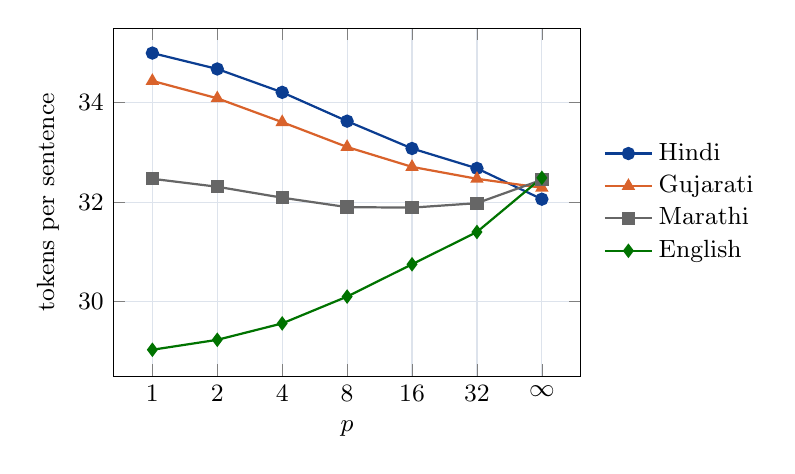
\begin{tikzpicture}
\begin{axis}[
  width=0.62\linewidth, height=6cm,
  xlabel={$p$}, ylabel={tokens per sentence},
  symbolic x coords={1,2,4,8,16,32,$\infty$}, xtick=data,
  ymin=28.5, ymax=35.5,
  grid=major, grid style={draw=soft},
  legend style={font=\small, at={(1.03,0.5)}, anchor=west, draw=none},
  legend cell align=left,
  tick label style={font=\small}, label style={font=\small}]
\addplot[mark=*, thick, color=pfair] coordinates
  {(1,35.00) (2,34.68) (4,34.21) (8,33.63) (16,33.08) (32,32.68) ($\infty$,32.06)};
\addplot[mark=triangle*, thick, color=hybrid] coordinates
  {(1,34.44) (2,34.09) (4,33.61) (8,33.11) (16,32.71) (32,32.47) ($\infty$,32.29)};
\addplot[mark=square*, thick, color=black!60] coordinates
  {(1,32.47) (2,32.31) (4,32.09) (8,31.90) (16,31.89) (32,31.98) ($\infty$,32.45)};
\addplot[mark=diamond*, thick, color=green!45!black] coordinates
  {(1,29.03) (2,29.23) (4,29.56) (8,30.10) (16,30.75) (32,31.40) ($\infty$,32.49)};
\legend{Hindi, Gujarati, Marathi, English}
\end{axis}
\end{tikzpicture}
\caption{Cost of the same sentence in each language as $p$ grows (values of
Table~\ref{tab:perlang}). The four costs converge.}
\label{fig:perlang}
\end{figure}

\begin{table}[t]
\centering
\caption{Parity and compression at a 32k vocabulary with English at four times the text of
each other language. Mean $\pm$ standard deviation over five samples of training text.
``Merges led by English'' is the share of merges to whose score English contributes most.}
\label{tab:front}
\begin{tabular}{lcccc}
\toprule
 & Gini of cost & \multicolumn{2}{c}{Compression (bytes/token)} & Merges led\\
\cmidrule(lr){3-4}
Tokenizer & (devtest) $\downarrow$ & training text $\uparrow$ & devtest $\uparrow$ & by English\\
\midrule
Classical ($p=1$) & $0.0380\pm0.0002$ & $6.910\pm0.004$ & $8.719\pm0.007$ & 49\%\\
$p=2$  & $0.0347\pm0.0002$ & $6.907\pm0.004$ & $8.761\pm0.006$ & 47\%\\
$p=4$  & $0.0298\pm0.0002$ & $6.897\pm0.004$ & $8.818\pm0.004$ & 43\%\\
$p=8$  & $0.0229\pm0.0002$ & $6.868\pm0.004$ & $8.868\pm0.005$ & 38\%\\
$p=16$ & $0.0152\pm0.0002$ & $6.818\pm0.005$ & $8.889\pm0.007$ & 34\%\\
$p=32$ & $0.0084\pm0.0001$ & $6.760\pm0.006$ & $8.882\pm0.004$ & 30\%\\
Parity-aware ($p=\infty$) & $0.0028\pm0.0004$ & $6.634\pm0.007$ & $8.830\pm0.006$ & 23\%\\
\midrule
Hybrid, 90\% classical & $0.0270\pm0.0002$ & $6.891\pm0.003$ & $8.788\pm0.005$ & 44\%\\
Hybrid, 75\% classical & $0.0180\pm0.0005$ & $6.827\pm0.004$ & $8.821\pm0.008$ & 37\%\\
Hybrid, 50\% classical & $0.0023\pm0.0004$ & $6.651\pm0.004$ & $8.834\pm0.005$ & 25\%\\
\bottomrule
\end{tabular}
\end{table}

\begin{figure}[t]
\centering
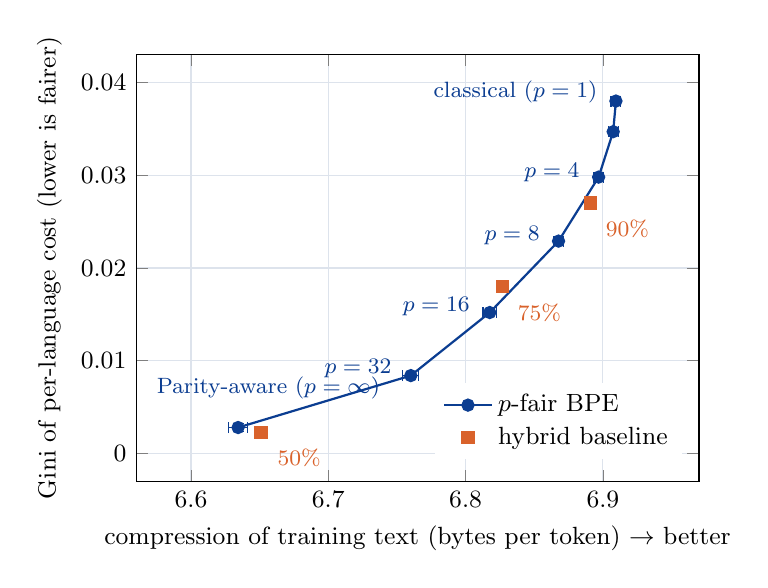
\begin{tikzpicture}
\begin{axis}[
  width=0.72\linewidth, height=7cm,
  xlabel={compression of training text (bytes per token) $\rightarrow$ better},
  ylabel={Gini of per-language cost (lower is fairer)},
  xmin=6.56, xmax=6.97, ymin=-0.003, ymax=0.043,
  xtick={6.6,6.7,6.8,6.9}, ytick={0,0.01,0.02,0.03,0.04},
  scaled y ticks=false,
  yticklabel style={/pgf/number format/fixed,/pgf/number format/precision=2},
  grid=major, grid style={draw=soft},
  legend style={font=\small, at={(0.97,0.05)}, anchor=south east, draw=none, fill=white},
  legend cell align=left,
  tick label style={font=\small}, label style={font=\small}]
\addplot[mark=*, mark size=2pt, thick, color=pfair,
  error bars/.cd, x dir=both, x explicit, y dir=both, y explicit]
  coordinates {
    (6.9095,0.0380) +- (0.0036,0.0002)
    (6.9075,0.0347) +- (0.0036,0.0002)
    (6.8969,0.0298) +- (0.0035,0.0002)
    (6.8677,0.0229) +- (0.0036,0.0002)
    (6.8176,0.0152) +- (0.0049,0.0002)
    (6.7601,0.0084) +- (0.0059,0.0001)
    (6.6343,0.0028) +- (0.0067,0.0004)
  };
\addplot[only marks, mark=square*, mark size=2.2pt, color=hybrid,
  error bars/.cd, x dir=both, x explicit, y dir=both, y explicit]
  coordinates {
    (6.6510,0.0023) +- (0.0039,0.0004)
    (6.8271,0.0180) +- (0.0039,0.0005)
    (6.8908,0.0270) +- (0.0034,0.0002)
  };
\legend{$p$-fair BPE, hybrid baseline}
\node[font=\footnotesize, text=pfair, anchor=east] at (axis cs:6.9030,0.0390) {classical ($p=1$)};
\node[font=\footnotesize, text=pfair, anchor=east] at (axis cs:6.8900,0.0303) {$p=4$};
\node[font=\footnotesize, text=pfair, anchor=east] at (axis cs:6.8610,0.0235) {$p=8$};
\node[font=\footnotesize, text=pfair, anchor=east] at (axis cs:6.8100,0.0159) {$p=16$};
\node[font=\footnotesize, text=pfair, anchor=east] at (axis cs:6.7530,0.0092) {$p=32$};
\node[font=\footnotesize, text=pfair, anchor=south west] at (axis cs:6.5680,0.0048) {Parity-aware ($p=\infty$)};
\node[font=\footnotesize, text=hybrid, anchor=north west] at (axis cs:6.8950,0.0262) {90\%};
\node[font=\footnotesize, text=hybrid, anchor=north west] at (axis cs:6.8310,0.0172) {75\%};
\node[font=\footnotesize, text=hybrid, anchor=north west] at (axis cs:6.6560,0.0016) {50\%};
\end{axis}
\end{tikzpicture}
\caption{The measured front. Each point is the mean of five samples of training text and
the bars are one standard deviation; most are smaller than the marker. Classical BPE is at
the top right, Parity-aware BPE at the bottom left, and increasing $p$ moves along the
curve. The hybrid baseline (percentage of classical merges) lies on the same curve.}
\label{fig:front}
\end{figure}

\subsection{The pattern is reliable}

Every increase in $p$ lowered both the Gini coefficient and the compression of the training
text in five of five samples. The standard deviation of the Gini coefficient across samples
is between 0.0001 and 0.0005, which is 10 to 30 times smaller than the difference between
neighbouring values of $p$. Resampling the test sentences gives the same conclusion: the
95\% interval for classical BPE is $[0.036,0.040]$ and for $p=8$ it is $[0.021,0.025]$, and
each step up in $p$ lowers the Gini coefficient in at least 99.7\% of the 1000 resamples.

\subsection{$p$-fair BPE matches the hybrid baseline and does not improve on it}

The hybrid points in Figure~\ref{fig:front} lie on the $p$-fair curve. To compare the
methods at equal compression we interpolate the $p$-fair curve at the compression of each
hybrid tokenizer, separately in each sample, and take the difference in Gini
(Table~\ref{tab:hybrid}). The differences are about 0.001, consistent in sign across the five
samples, and go in both directions: $p$-fair is slightly fairer at 75\%, the hybrid is
slightly fairer at 50\% and 90\%. Neither method dominates. The hybrid with 50\% classical
merges is at least as good as pure Parity-aware BPE on both measures (0.0023 against 0.0028
in Gini, 6.65 against 6.63 in compression), in line with the motivation for the hybrid
in \cite{foroutan2026}.

The two methods do distribute cost differently (Table~\ref{tab:perlang}). The hybrid's
parity phase equalises the three Indian languages with one another, which raises Marathi
above its cost under classical BPE (33.3 against 32.5 tokens at 75\%). $p$-fair BPE at
similar compression keeps Marathi below its classical cost (31.9 at $p=8$) and leaves a
wider spread between the Indian languages. Which behaviour is preferable depends on whether
the aim is equal cost or no language made worse off.

\begin{table}[t]
\centering
\caption{Hybrid baseline against $p$-fair BPE at the same training-text compression.
Difference in Gini (hybrid minus $p$-fair), mean $\pm$ standard deviation over five samples.}
\label{tab:hybrid}
\begin{tabular}{lcc}
\toprule
Hybrid & Gini difference & Fairer method (samples)\\
\midrule
90\% classical & $-0.0014\pm0.0004$ & hybrid (5 of 5)\\
75\% classical & $+0.0013\pm0.0003$ & $p$-fair (5 of 5)\\
50\% classical & $-0.0012\pm0.0005$ & hybrid (5 of 5)\\
\bottomrule
\end{tabular}
\end{table}

\subsection{The disparity depends on data balance, and less on vocabulary size}

Table~\ref{tab:sens} repeats the experiment with other amounts of English and with a larger
vocabulary. These are single runs. The direction is the same in every setting: the Gini
coefficient and the compression fall at every step. The size of the problem changes a great
deal. With equal amounts of text classical BPE is already close to parity (Gini 0.019), and
the cost of full parity is 1.1\% of compression. With eight times as much English the Gini
coefficient is 0.051, a Hindi sentence costs 30\% more tokens than its English translation,
and full parity costs 7.0\%.

With equal data the remaining disparity is not between English and the Indian languages:
English (31.7 tokens) lies between Marathi (30.4) and Hindi (33.3).

Doubling the vocabulary to 64k leaves the Gini coefficient of classical BPE unchanged
(0.038) and that of Parity-aware BPE unchanged (0.003). We therefore do not observe, between
these two sizes, the widening reported for larger vocabularies in \cite{lee2026}.

\begin{table}[t]
\centering
\caption{Gini coefficient in other settings, and the compression lost by going from
classical to Parity-aware BPE. The row marked $\dagger$ is the five-sample mean of
Table~\ref{tab:front}; the others are single runs.}
\label{tab:sens}
\begin{tabular}{llcccccc}
\toprule
English & Vocab. & $p=1$ & $p=2$ & $p=4$ & $p=8$ & $p=\infty$ & Cost of parity\\
\midrule
$1\times$ & 32k & 0.0186 & 0.0172 & 0.0148 & 0.0117 & 0.0034 & 1.1\%\\
$4\times$ $\dagger$ & 32k & 0.0380 & 0.0347 & 0.0298 & 0.0229 & 0.0028 & 4.0\%\\
$8\times$ & 32k & 0.0505 & 0.0461 & 0.0383 & 0.0298 & 0.0033 & 7.0\%\\
$4\times$ & 64k & 0.0378 & 0.0353 & 0.0313 & 0.0255 & 0.0032 & 5.1\%\\
\bottomrule
\end{tabular}
\end{table}

\subsection{The cost unit decides the outcome}\label{sec:unitresult}

Table~\ref{tab:byte} shows what happens when cost is measured per byte, as in our first
formulation. English is then the ``worst-off'' language, and the parity rule gives it 99\%
of the merges. Measured by what a user pays, the result is the opposite of the intention:
the Indian languages need about twice as many tokens per sentence as before, and English
needs fewer. This is why Section~\ref{sec:unit} uses parallel sentences.

\begin{table}[t]
\centering
\caption{Tokens per sentence when the training cost is measured per byte (single run).}
\label{tab:byte}
\begin{tabular}{lcccc}
\toprule
Tokenizer & Hindi & Marathi & Gujarati & English\\
\midrule
Classical BPE & 35.0 & 32.5 & 34.4 & 29.0\\
Parity-aware BPE, cost per byte & 63.6 & 70.6 & 66.5 & 26.6\\
\bottomrule
\end{tabular}
\end{table}

\subsection{Compression on balanced test text}

On devtest, where every language has the same amount of text, intermediate values of $p$
compress \emph{better} than classical BPE (8.89 bytes per token at $p=16$ against 8.72;
Table~\ref{tab:front}). Classical BPE optimises compression of the training mixture, which
is mostly English; a balanced test set rewards the vocabulary that $p$-fair BPE moves to
the other three languages. The trade-off in Figure~\ref{fig:front} is therefore a trade-off
against compression of the training distribution, and whether it is a real cost depends on
the mixture of languages the tokenizer will meet in use.

% \subsection{Training time}

% On a two-core machine a 32k tokenizer trains in about 15 seconds on 140 million characters,
% against about 5 minutes with full rescoring. The lazy heap re-checks on average 3 entries
% per merge at $p=1$ and 30 at $p=8$.

% =====================================================================
\section{Challenges and limitations}

\begin{itemize}
  \item \textbf{No advantage over the hybrid baseline.} On this front $p$-fair BPE and the
  hybrid schedule are equivalent. What $p$-fair BPE offers is a single rule derived from
  one objective, and a different distribution of cost between languages. An advantage in
  the numbers would have to come from the morphology penalty or the budget allocation.
  \item \textbf{The disparity is partly a design choice.} With four languages, three of
  them closely related, the gap comes mainly from how much English is in the training text.
  The $4\times$ setting is an assumption, and the results should be read with
  Table~\ref{tab:sens} in mind.
  \item \textbf{Small scale.} The training text is 140 million characters, the test set is
  1012 sentences, and the sensitivity runs are single runs.
  \item \textbf{Re-implemented baselines.} Parity-aware BPE and the hybrid are our
  implementation, character-level and without the moving-window variant.
  \item \textbf{Greedy, first-order steps.} Proposition~\ref{prop:rule} is a first-order
  argument, and greedy merging carries no optimality guarantee for $p>1$. The measured
  curve is the curve of the greedy algorithm, not the Pareto front of \eqref{eq:obj}.
  \item \textbf{Lazy evaluation with the morphology penalty.} In \eqref{eq:morph} both the
  count and the penalty of a pair fall over time, so the score is no longer guaranteed to be
  non-increasing and Proposition~\ref{prop:lazy} needs a modified bound when $\lambda>0$.
  \item \textbf{Morphology and downstream quality.} Alignment with morphemes explains little
  of downstream performance \cite{arnett2025}, so it has to be reported as its own axis and
  checked against a task.
  \item \textbf{Shared budget within a script.} Hindi and Marathi share the Devanagari
  budget in \eqref{eq:alloc}, so parity between them rests on the $p$-fair rule alone.
\end{itemize}

% =====================================================================
\section{Work ahead}

\begin{enumerate}
  \item \textbf{Morphology.} Implement the penalty of \eqref{eq:morph} with SuTRA
  boundaries, sweep $(p,\lambda)$, and report boundary F1 and the hypervolume of the
  three-axis front.
  \item \textbf{Scaling.} Extend to a 128k vocabulary to test whether intermediate $p$
  avoids the loss of equity reported for Parity-aware BPE at large vocabularies
  \cite{lee2026}.
  \item \textbf{Allocation.} Fit the cost curves $t_c(k)$ per script, solve
  \eqref{eq:alloc}, and compare with the union-proportion rule \cite{brahma2026} and a
  uniform split.
  \item \textbf{Downstream evaluation.} Hindi--Marathi translation (chrF++) and the number
  of tokens per technical term, to test whether the intrinsic gains matter in use.
  \item \textbf{Extension.} A $p$-fair version of Unigram vocabulary pruning
  \cite{kudo2018}.
\end{enumerate}

% =====================================================================
\section{Conclusion}

Classical BPE and Parity-aware BPE are the two ends of one family: the greedy step of a
power-mean objective, with the exponent $p$ as the dial. The family can be trained exactly
and quickly, and on Hindi, Marathi, Gujarati and English it traces a smooth and repeatable
curve from maximum compression to equal cost, on which most of the disparity can be removed
for well under one per cent of compression. The curve is the same as that of the existing
hybrid schedule, so the contribution so far is a principled formulation and a careful
measurement, and not a better tokenizer. Whether the formulation leads to one depends on
the two components that remain: the morphology penalty and the convex budget allocation.

% =====================================================================
\begin{thebibliography}{99}\small

\bibitem{arnett2025}
C.~Arnett, M.~Hudspeth, and B.~O'Connor.
\newblock Evaluating morphological alignment of tokenizers in 70 languages.
\newblock arXiv:2507.06378, 2025.

\bibitem{boyd2004}
S.~Boyd and L.~Vandenberghe.
\newblock \emph{Convex Optimization}.
\newblock Cambridge University Press, 2004.

\bibitem{brahma2026}
M.~Brahma, N.~J. Karthika, R.~Verma, N.~S. Naidu, R.~Saluja, M.~S. Desarkar, and G.~Ramakrishnan.
\newblock Multilingual tokenization through the lens of Indian languages: Challenges and insights.
\newblock In \emph{Findings of the Association for Computational Linguistics: ACL 2026}, pages 32614--32632, 2026.

\bibitem{foroutan2026}
N.~Foroutan, C.~Meister, D.~Paul, J.~Niklaus, S.~Ahmadi, A.~Bosselut, and R.~Sennrich.
\newblock Parity-aware byte-pair encoding: Improving cross-lingual fairness in tokenization.
\newblock In \emph{Proceedings of the 64th Annual Meeting of the Association for Computational Linguistics (Volume 1: Long Papers)}, pages 7514--7538, 2026.

\bibitem{gage1994}
P.~Gage.
\newblock A new algorithm for data compression.
\newblock \emph{The C Users Journal}, 12(2):23--38, 1994.

\bibitem{khan2024}
M.~S.~U.~R. Khan, P.~Mehta, A.~Sankar, U.~Kumaravelan, S.~Doddapaneni, Suriyaprasaad~B, Varun~G, S.~Jain, A.~Kunchukuttan, P.~Kumar, R.~Dabre, and M.~M. Khapra.
\newblock IndicLLMSuite: A blueprint for creating pre-training and fine-tuning datasets for Indian languages.
\newblock In \emph{Proceedings of the 62nd Annual Meeting of the Association for Computational Linguistics (Volume 1: Long Papers)}, pages 15831--15879, 2024.

\bibitem{kudo2018}
T.~Kudo.
\newblock Subword regularization: Improving neural network translation models with multiple subword candidates.
\newblock In \emph{Proceedings of the 56th Annual Meeting of the Association for Computational Linguistics (Volume 1: Long Papers)}, pages 66--75, 2018.

\bibitem{lee2026}
K.~S.~J.~W. Lee, M.~R. Qorib, A.~I. Soegeng, and H.~T. Ng.
\newblock Equity with efficiency: An empirical study of tokenizers for multilingual large language models.
\newblock arXiv:2606.15044, 2026.

\bibitem{minoux1978}
M.~Minoux.
\newblock Accelerated greedy algorithms for maximizing submodular set functions.
\newblock In \emph{Optimization Techniques}, Lecture Notes in Control and Information Sciences, vol.~7, pages 234--243. Springer, 1978.

\bibitem{nllb2022}
NLLB Team.
\newblock No language left behind: Scaling human-centered machine translation.
\newblock arXiv:2207.04672, 2022.

\bibitem{petrov2023}
A.~Petrov, E.~La~Malfa, P.~Torr, and A.~Bibi.
\newblock Language model tokenizers introduce unfairness between languages.
\newblock In \emph{Advances in Neural Information Processing Systems 36 (NeurIPS 2023)}, 2023.

\bibitem{rathore2026}
V.~Rathore, S.~Gole, D.~Telwadkar, R.~Bhatia, M.~Ruparel, S.~Sureka, and N.~Bhargava.
\newblock SuTRA: Structurally-unified tokenization with root awareness.
\newblock arXiv:2608.18087, 2026.

\bibitem{sennrich2016}
R.~Sennrich, B.~Haddow, and A.~Birch.
\newblock Neural machine translation of rare words with subword units.
\newblock In \emph{Proceedings of the 54th Annual Meeting of the Association for Computational Linguistics (Volume 1: Long Papers)}, pages 1715--1725, 2016.

\bibitem{zouhar2023}
V.~Zouhar, C.~Meister, J.~Gastaldi, L.~Du, T.~Vieira, M.~Sachan, and R.~Cotterell.
\newblock A formal perspective on byte-pair encoding.
\newblock In \emph{Findings of the Association for Computational Linguistics: ACL 2023}, pages 598--614, 2023.

\end{thebibliography}

\end{document}